\section{Methodology}
\subsection{Description of data sources}
The data used by the information system is sourced from three public registers:
\begin{enumerate}
	\item The Central Insolvency Register (\textit{Centraal Insolventie Register or CIR})
	\item The Register of lawyers (\textit{NOvA's Tableau}) 
	\item The Register of ancillary positions of judges. (\textit{Register van nevenfuncties van rechters}) 
\end{enumerate}
	
The CIR provides the bulk of the data. The other two registers are used for the entity resolution of administrators and judges.

\subsubsection{Central Insolvency Register}
\paragraph{Introduction}
The CIR \cite{rechtspraak:1} contains company insolvency data supplied by the courts and the administrators. Courts are obliged to supply the insolvency data and free consultation of thereof according to the insolvency law, article 19 \cite{law:1}. CIR started the register on the 1st of January 2005 and retains case related data until six months after the ending of the insolvency. 

\paragraph{SOAP web service}
CIR operates a web service using the HTTP SOAP 1.2 protocol which returns information in XML format. Using the web service we can request the new and updated entities of:

\begin{itemize}
	\item Insolvents
	\item Publications, by the Court
	\item Reports, by the Administrator (meta data only)
	\item Judges 
	\item Administrators
	\item Courts
\end{itemize}

\begin{figure}[h]
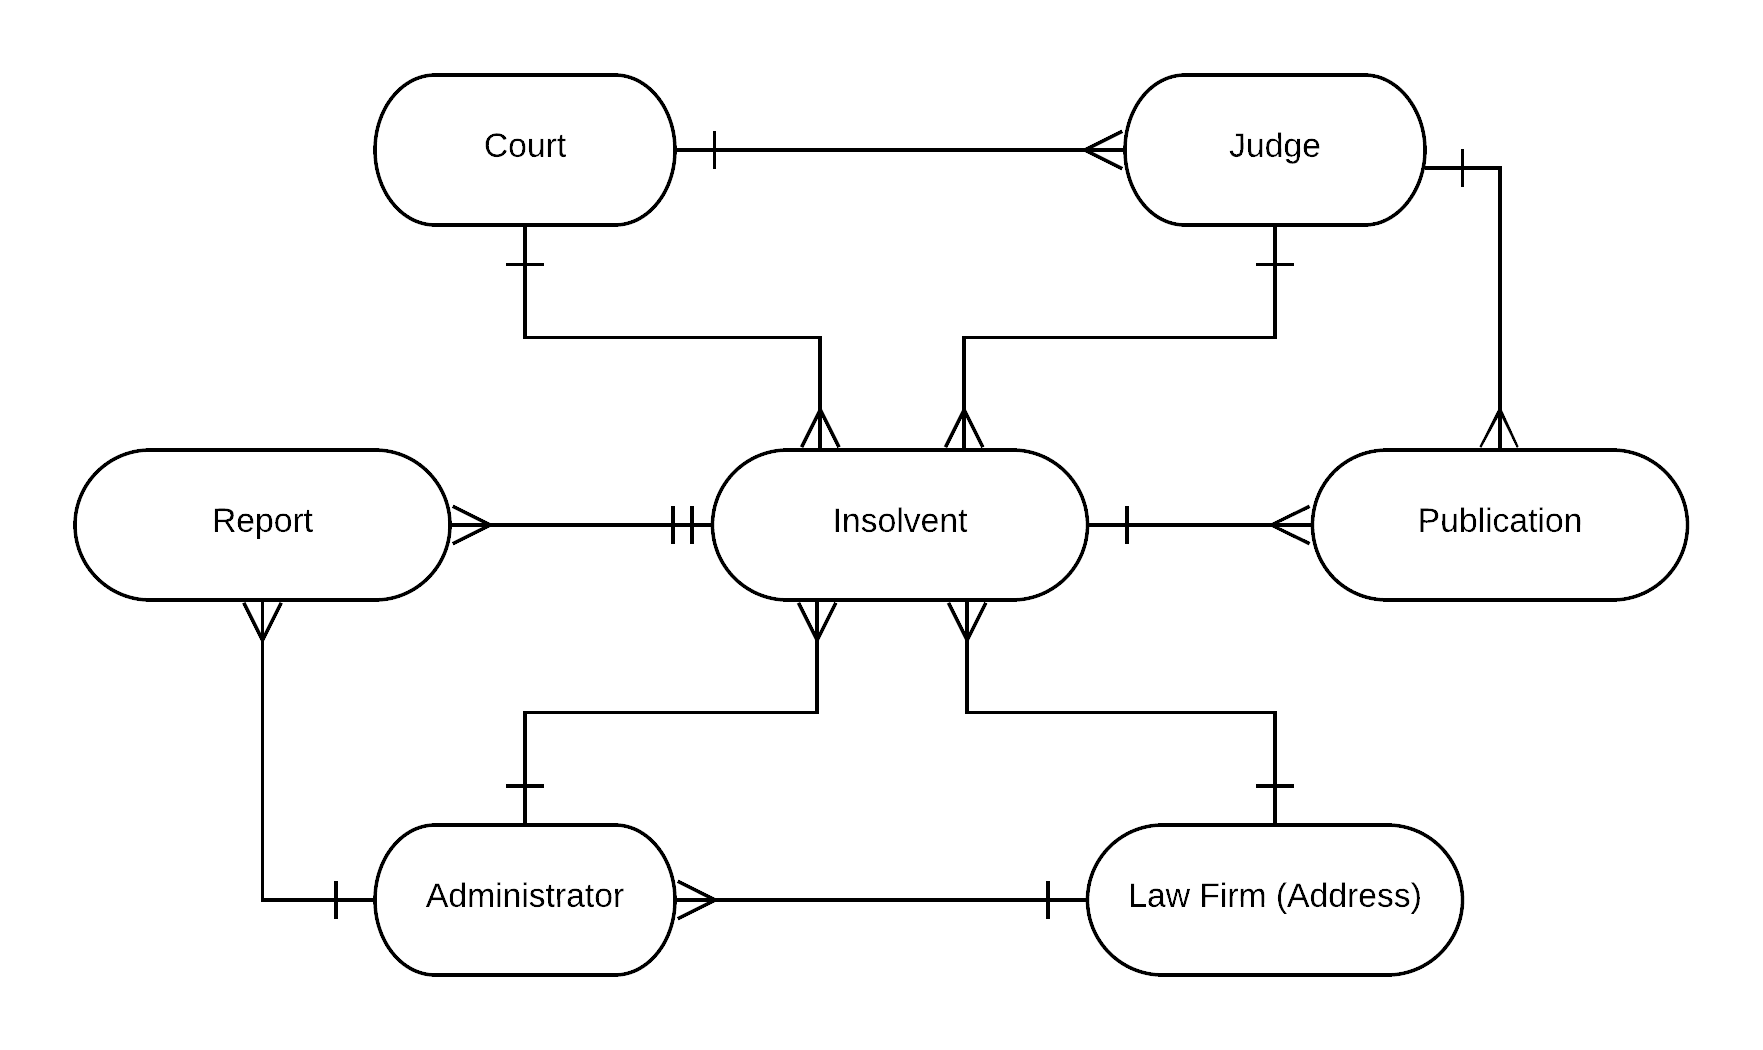
\includegraphics[width=1\linewidth]{cir_erd.png}
\caption{Insolvency entity relations.}
\end{figure}

The returned XML data is structured: the entities are connected in the XML response by composition as defined in XSD schemas provided by CIR. Unique identifiers exist for the Insolvent, Publication and Report entities and they can easily be stored in normalized SQL tables. 

\paragraph{Database normalization}
Not all the data is normalized. The entities Judges and Administrators have no identifiers but consist of free text fields for their name parts. This leads to unwanted duplication as names can be written in many different forms and typos can be introduced, e.g. one judge's name appears as:

\begin{itemize}
\item "mr. W.J. Geurts - de Veld"
\item "mr. W.J. Geurts-deVeld"
\item "mr. W.J. Geurts-de Veld"
\item "mr. W.J.Geurts-de Veld"
\item "mr.W.J. Geurts-de Veld"
\item "mr. W.J. Geurts-de Veld (Rotterdam)"
\item "mr W.J.Geurts-de Veld"
\item "W.J.Geurts-de Veld"
\end{itemize}

We need to define so-called master data for judges and administrators containing the real world entities. The two data sources in the sections \ref{NOvA Tableau} and \ref{Nevenfuncties Rechters} are chosen for this purpose. CIR entity names are first normalized for de-duplication and are subsequently linked to the master data records on their normalized name. 

\paragraph{PDF report web service}
A second web service operated by CIR provides Administrator Reports in PDF format by HTTP request. There are two types of reports: 
\begin{enumerate}
\item progress reports
\item financial attachments
\end{enumerate}
Recofa has published templates for both report types\cite{rechtspraak:3}. These reports hold much of the unstructured data.

\paragraph{CIR data contents}
Table \ref{table:cir_contents} shows the content of the CIR register data as of date [2018-08-12] and the average monthly size of new additions.

\begin{table}[h]
\caption{Actual number of records and monthly average additions per entity.}
\centering
\begin{tabular}{l r r}
\hline\hline
Entity & no. of records & monthly add.\\
\hline
Insolvent & 17,331 & 280 \\
Report & 146,865 & 4408 \\
... progress report & 87,430 &  \\
... financial attachment. & 56,611 &  \\
Publication & 37,031 & 1447 \\
Administrator (distinct) & 2329 & \\
Judge (distinct) & 451 & \\
Court & 11 & \\
\hline
\end{tabular}
\label{table:cir_contents}
\end{table}

The number of current defaults is about the lowest of the century [ref] [graph of declining defaults]

\subsubsection{Register of lawyers, NOvA Tableau}\label{NOvA Tableau}

The NOvA tableau is the official register for lawyers and maintained by the \textit{Nederlandse Orde van Advocaten (NOvA)}\cite{nova:1}. Lawyers are obliged to be registered in the tableau by the lawyer's law (\textit{advocatenwet}, article 1 \cite{law:2}). NOvA offers an on-line search form where key word search and filters can be applied to search for a lawyer. This data source is used to collect the master data for Administrators. 

\subsubsection{Register of judges, Nevenfuncties van rechters}\label{Nevenfuncties Rechters}

The Register for ancillary positions for judges is made available by \textit{de Rechtspraak}\cite{rechtspraak:2}. It offers an on line form and returns the name, current and historical occupation and ancillary positions. This data source is used to collect the master data for Judges.


\subsection{Description of the system and data flow}
\subsubsection{System components}
Figure \ref{System overview} gives an overview of the system components for extracting, enriching and integrating the sourced data and making the resulting structured and higher level information available to the user.

\begin{figure}[h]
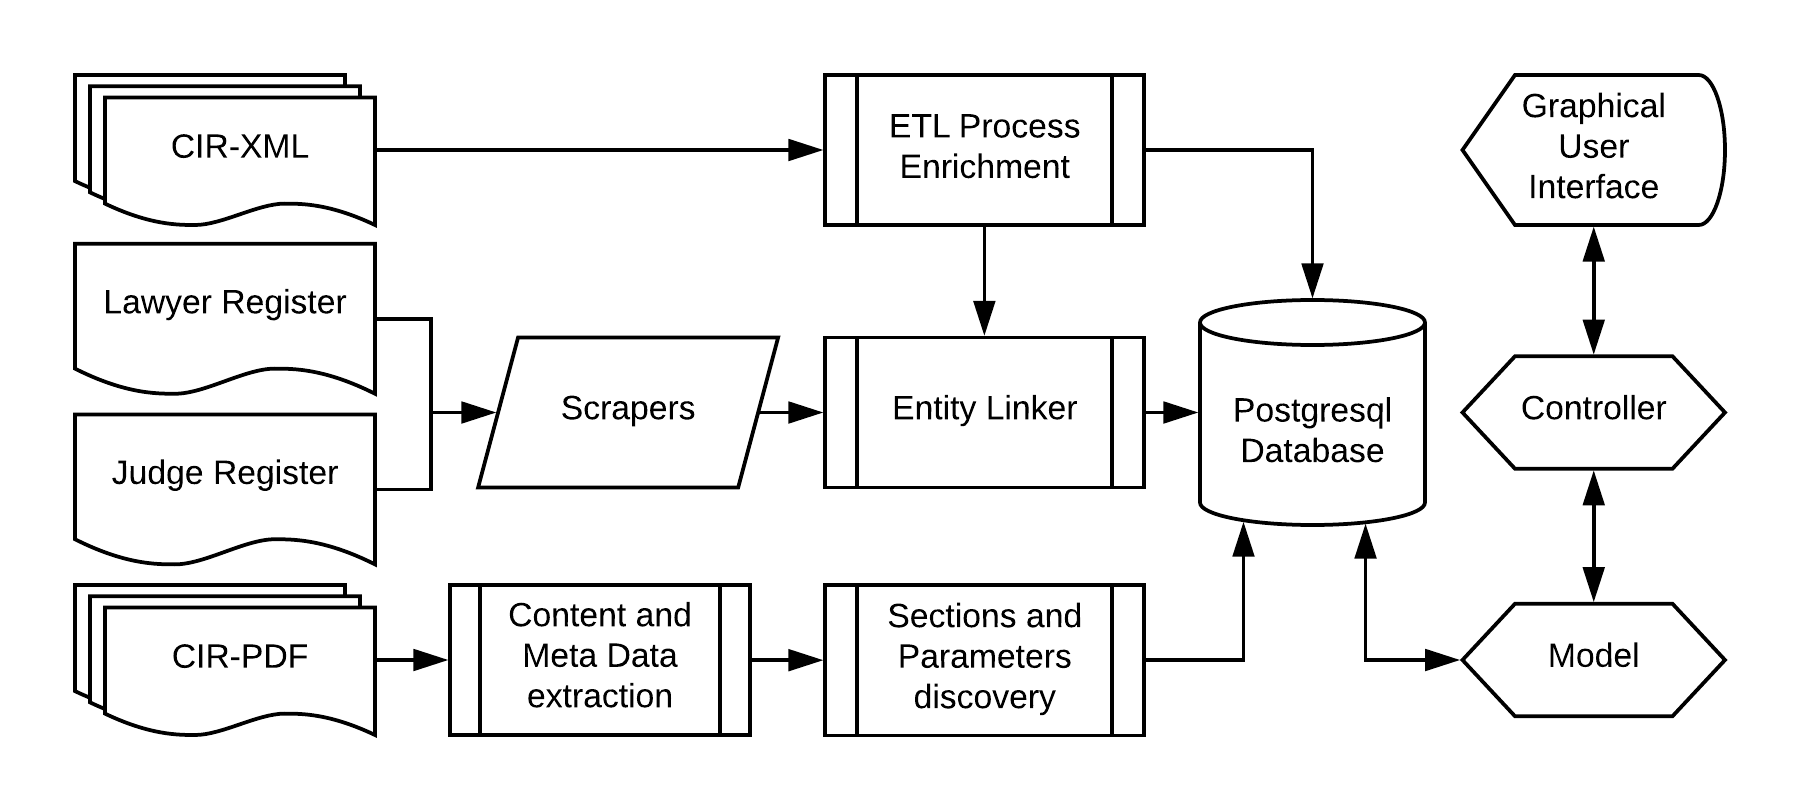
\includegraphics[width=1\linewidth]{system_overview.png}
\caption{System overview.}\label{System overview}
\end{figure}

\paragraph{The ETL process and Enrichment} This component extracts the entities with selected data fields from the XML. The data is enriched and annotated after which it is stored in the Postgresql database. An example of the enrichment are the start and end date of the insolvency which are derived from court publications.

\paragraph{The Entity Linker} This component is responsible for linking judges and administrators in CIR to real life entities found in the judge and lawyer registers. It does this by normalization of the CIR names and resolving them to the register entities using similarity functions. Unresolved entities can be linked manually to guarantee completeness. Established links are stored in an association table. After an initial run, the register scrapers are called upon only when new judges or administrators entries appear in CIR.

\paragraph{PDF processors}
PDF reports are processed to extract the textual content and meta data. The text sections, as defined in the progress report template, and key data parameter are discovered in a subsequent process. This data is available for search later on.

\paragraph{Model-View-Controller (MVC)}
This is a well established pattern of three subcomponents working together for a GUI. The user operates a graphical interface, prototyped in Jupyter notebooks, to query the data or interact with data visualisations or tables. The interface is the View in the MVC component. On user command, the Controller asks the Model to prepare the necessary data and then passes this data to the View to update the interface.


\subsection{Implementation challenges}
\subsubsection{Entity De-duplication, Scraping and Linking}
\paragraph{Deduplication: normalizing names}
CIR provides administrator names in four parts: title, initials, middle part and family name. 

\textbf{The initials} were normalized into single characters using periods and no spaces. In Dutch, initials for names like \textit{Theodoor} and \textit{Christiaan} are written with two or three characters as \textit{Th.} or \textit{Chr.}. These names are derived from the Greek where the initial \textit{Th(eta)} for example is written as one character. Initials for double names like \textit{Albert-Jan} may be written as \textit{A-J.} or \textit{A.-J.}. 

\textbf{The middle part}, e.g. 'van der' or 'ter' was sometimes supplied in the middle part field and sometimes in the family name (and sometimes in both). To normalize the middle part it was merged into the family name making sure it did not appear twice.

\textbf{The family name} was stripped from academic and noble (not uncommon in this profession) titles. Misplaced initials and CIR specific comments were removed. Maiden names are connected to the surname with a hyphen and no spaces.

Furthermore, all parts are made lower case, surrounding whitespace characters are stripped, accents are removed and multiple spaces are replaces with a single space. 

De-duplication by normalizing the administrator names reduced the number of distinct administrator names from 2329 to 1559, a 33\% reduction.
\\\\
Judge names are provided in a single field. This sometimes leads to initials or a middle name part that is stuck together to the family name and was separated using regexm e.g. in 'C. vanSteenderen' and 'mr. W.J.Geurts-de Veld'. CIR often adds the court between parenthesis which was also removed in the normalization.

De-duplication by normalizing the judge names reduced the number of distinct judge names from 565 to 277, a 51\% reduction.

\paragraph{Administrator name scraping}
NOvA unfortunately does not provide complete lists of registered lawyers to which we could link the administrators. Instead we link the administrator by using the site's search form. An underlying REST API returning JSON data was discovered which was used instead of the form. The API (or form) can not handle initials or stop words as 'de' and 'van' and only the family name without stop words was used. The best candidate in the search results, which are sorted on the relevance provided by NOvA, is found by (partially) matching the initials until a match is found. The API enables the use of filters and we filter from narrow to broad until a candidate is found, filtering on: 
\begin{enumerate}
\item{legal specialism: administrator}
\item{legal branch: insolvency law}
\item{no filter}
\end{enumerate}

NOvA only supplies the actual lawyer register but CIR also lists administrators previously working on a case therefore a substantial amount of administrators cannot be linked. Another website, www.advocatenzoeken.nl that sources data from NOvA but keeps historical data was scraped as well to complement NOvA.

\paragraph{Administrator name linking}
From the normalized name list we linked 73\% to NOVa registered lawyers and another 18\% administrators from the www.advocatenzoeken.nl site. The remaining 10\% unfound names are linked to a special 'unknown' lawyer.

\begin{table}[h]
\caption{Administator entity linking results}
\centering
\begin{tabular}{l r r r}
\hline\hline
Source & no. linked & correct & incorrect\\
\hline
NOvA & 1134 & 1133 & 1\\
AdvocatenZoeken & 280 & 279 & 1 \\
Not found & 149 &&\\
\hline
Total & 1563 & 1412 &\\
\hline
\end{tabular}
\label{table:administrator_linking}
\end{table}

Correctness is assumed when the names match. When an obvious typo is found in the family name. When the initials either match, or are contained in the master record or are permutated or are missing. 

[discuss not found results: common name, place in name]

\paragraph{Judge name scraping}
The CIR register for ancillary functions for judges was scraped for judges from courts and higher courts. The total set contains 3691 judges and should be a superset of active case judges. The website was driven by the Angular javascript framework and could not easily be scraped with simple HTTP requests. Selenium was used to mimic user browsing behaviour to invoke the javascript. 

\paragraph{Judge entity linking}
A judge is linked by to a judge master record with the most similar normalized name where similarity was calculated using the Levensthein or edit distance. 88\% of the normalized names were matched. 4 of the incorrectly 12\% matched names could be set manually and the remaining 8\% was linked to a special 'unknown' judge.


\begin{table}[h]
\caption{Judge entity linking results}
\centering
\begin{tabular}{l r r r}
\hline\hline
Source & no. linked & correct & incorrect\\
\hline
Ancillary positions register & 277 & 246 & 32\\
+Manual lookup of the 32 &   & 10 & -10\\
\hline
Total & 277 & 256 & 22\\
\hline
\end{tabular}
\label{table:judge_linking}
\end{table}

Correctness is defined similar to the administrator normalized name correctness.

[discuss not found (initially) results: maiden name, not a judge anymore]

\subsubsection{Process Mining}

\subsubsection{PDF content extraction}
The PDF reports can be split into two types depending on how the PDF was created:
\begin{enumerate}
\item Scanned from paper using a scanner or copier.
\item Converted by software from another format.
\end{enumerate}

\paragraph{Scanned PDFs}
Scanned PDFs contain images only. To convert the images to text we used the Ghostscript library for image extraction and the Tesseract OCR engine for the character recognition. Tesseract supports the Dutch language which is paramount to our application. It is very important to supply Tesseract with good quality images. We used the Ghostscript settings of a \emph{tiffgray} output device with a \emph{300 DPI} resolution. 

\paragraph{Converted PDFs}
Converted PDF content can be extracted with a number of packages such as PDFMiner, PyPDF2, pyPoppler and pdftotext. We chose the latter after comparison because it maintains the layout which is important for section and parameter extraction and being build in C++ it is very fast.

\paragraph{Third type}
A third type appeared: PDFs that were scanned and subsequently OCR-ed by a copier. They contain both text and images. The OCR quality is often poor. We retried re-OCR-ing the images with Tesseract which solved some errors but introduced others. Meta data about a.o. the scanner type was obtained which could improve post-process text extraction in future work.


\subsubsection{PDF report section and parameter extraction}
[todo]



